\begin{frame}{Origins of Molecular Dynamics (MD)}
    \begin{itemize}
        \item Modern MD was developed in the 1950s, influenced by Monte Carlo methods popularized at Los Alamos National Laboratory.
        \pause
        \bigskip
        \item However, interest in the evolution of N-body systems dates back to the 17th century with Isaac Newton, focusing mainly on celestial mechanics.
        \pause
        \bigskip
        \item Many key numerical algorithms were created before computers. For example, the \textbf{Verlet integration algorithm}, the most common today, was used as early as 1791 by Jean Baptiste Joseph Delambre.
    \end{itemize}
\end{frame}

\begin{frame}{Pre-Computational Methods}
    Before digital computers, modeling was done in other ways:
    \pause
    
    \begin{itemize}
        \item \textbf{Analog computers} were used to integrate the equations of motion.
        \pause
        \item Some scientists built \textbf{physical models} with spheres to replicate the structure of liquids and study their behavior.
    \end{itemize}
    \pause
    
    \begin{block}<4->{The Fermi-Pasta-Ulam-Tsingou Problem}
        To understand the origin of irreversibility, Enrico Fermi and his collaborators used the \textbf{MANIAC I} computer in 1953 to simulate the time evolution of a many-body system.
    \end{block}
\end{frame}

\begin{frame}{FPU Problem Graph}
    \begin{figure}
        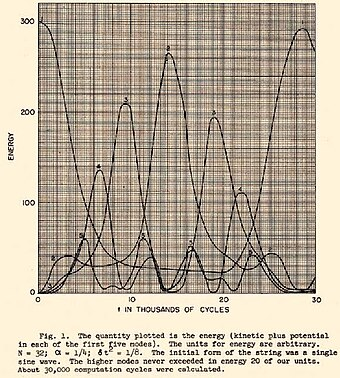
\includegraphics[width=0.5\textwidth]{images/MANIAC.png}
        \caption{Energy vs. time for one of the first N-body systems simulated by Fermi, showing unexpected and non-irreversible behavior.}
    \end{figure}
\end{frame}

\begin{frame}{Towards Realistic Matter Simulations}
    \footnotesize
    With the advent of more powerful computers, simulations became more realistic:
    \pause
    
    \begin{itemize}
        \item \textbf{1957:} Alder and Wainwright simulated elastic collisions between hard spheres using an IBM 704 computer.
        \pause
        \bigskip
        \item \textbf{1960:} Gibson and his team performed perhaps the first realistic simulation, modeling radiation damage in solid copper.
        \pause
        \bigskip
        \item \textbf{1964:} Rahman simulated liquid argon using a \textbf{Lennard-Jones potential}, with results that agreed well with experimental data.
    \end{itemize}
    \pause
    
    \begin{alertblock}<4->{The Legacy of the Lennard-Jones Potential}
        Today, it remains one of the most widely used potentials for describing simple substances and as a component of more complex force fields.
    \end{alertblock}
\end{frame}

\begin{frame}{The Molecular Dynamics Algorithm: Key Steps}
    \begin{block}{Algorithm Steps}
        \begin{enumerate}
            \item \textbf{Initialization:} Initial positions and velocities are assigned to the atoms.
            \pause
            \item \textbf{Force Calculation:} The forces on each atom are calculated, either from classical ($F = -\nabla V(\vec{r})$) or quantum ($F = F(\Psi(\vec{r}))$) potentials.
            \pause
            \item \textbf{Integration:} Positions and velocities are updated for a small time step ($\Delta t$) using an integrator.
            \pause
            \item \textbf{Iteration:} Steps 2 and 3 are repeated for the time required to observe the system's evolution.
        \end{enumerate}
    \end{block}
\end{frame}

\begin{frame}{MD Algorithm Graph}
    \begin{figure}
        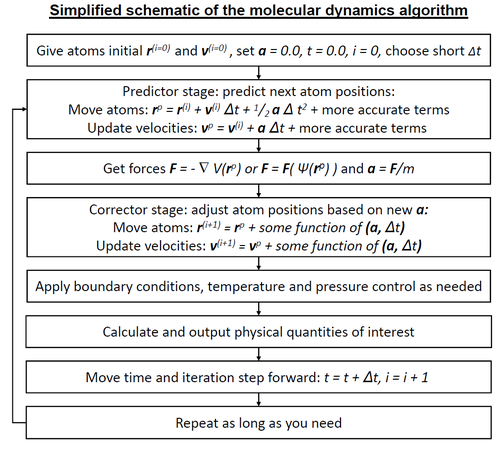
\includegraphics[width=0.5\textwidth]{images/algorithm.png}
        \caption{Simplified schematic of the Molecular Dynamics algorithm.}
    \end{figure}
\end{frame}

% --- START OF THE NEW SECTION ---

\begin{frame}{From Classical to Quantum MD}
    Let's recall the key step in the MD algorithm:
    \pause
    \begin{center}
        \large \textbf{Calculate the Forces}
    \end{center}
    \pause
    
    \begin{itemize}
        \item In classical MD, forces come from \textbf{predefined potentials} (force fields) like the Lennard-Jones potential.
        \pause
        \bigskip
        \item These potentials are efficient, but they \textbf{cannot describe} quantum phenomena like the formation or breaking of chemical bonds, or reactions.
        \pause
        \bigskip
        \item The natural question was: Can we calculate the forces directly from quantum mechanics \textbf{"on the fly"} at each step of the simulation?
    \end{itemize}
    \pause
    
    \begin{alertblock}<6->{The Birth of Quantum Molecular Dynamics}
        This idea gives rise to \textbf{Ab Initio Molecular Dynamics (AIMD)}, where forces are obtained by solving the Schrödinger equation for the electrons at each atomic configuration.
    \end{alertblock}
\end{frame}

%------------------------------------------------

\begin{frame}{The Breakthrough: The Car-Parrinello Method (1985)}
    The field of AIMD was revolutionized by a paper from \textbf{Roberto Car and Michele Parrinello}.
    \pause
    
    \begin{block}{The Car-Parrinello Innovation (CPMD)}
        \begin{itemize}
            \item Instead of fully solving for the electronic state at each step (which is very expensive), they introduced a \textbf{fictitious dynamics} for the electronic orbitals.
            \pause
            \item This unified the evolution of the nuclei (classical) and the electrons (quantum) into a \textbf{single Lagrangian dynamical system}.
            \pause
            \item It allowed for much longer and more efficient simulations than previous methods, opening the door to the study of complex systems in chemistry and materials science.
        \end{itemize}
    \end{block}
    \pause
    
    \begin{exampleblock}<4->{Impact}
        The Car-Parrinello method turned quantum molecular dynamics into a practical and predictive tool, and it remains one of the pillars of the field today.
    \end{exampleblock}
\end{frame}

%------------------------------------------------

\begin{frame}{Two Main Approaches in AIMD}
    From these developments, two main families of Quantum Molecular Dynamics emerged:
    \pause
    
    \begin{columns}
        \begin{column}{0.5\textwidth}
            \begin{block}{Born-Oppenheimer Molecular Dynamics (BOMD)}
                \begin{itemize}
                    \item Strictly adheres to the Born-Oppenheimer approximation.
                    \item \textbf{Calculates the electronic ground state} accurately at each time step.
                    \item It is conceptually simpler and very robust.
                    \item It generally allows for larger time steps, but each step is more computationally expensive.
                \end{itemize}
            \end{block}
        \end{column}
        \begin{column}{0.5\textwidth}
            \begin{block}{Car-Parrinello Molecular Dynamics (CPMD)}
                 \begin{itemize}
                    \item Propagates the nuclei and electronic orbitals simultaneously.
                    \item The electrons are \textbf{not exactly in the ground state} at each step, but they remain close to it.
                    \item It is computationally more efficient per time step.
                    \item It requires smaller time steps to maintain adiabaticity.
                \end{itemize}
            \end{block}
        \end{column}
    \end{columns}
\end{frame}

% --- END OF THE NEW SECTION ---